\chapter[Wheelchair locomotion]{Analysis of manual wheelchair locomotion}
\label{locomotion_analysis}

\section{Introduction}
Wheelchair locomotion concerns many people, for different reasons: genetic example: (myopathy), accidental (spinal cord injury, lower extremity amputee), degenerative (multiple sclerosis, poliomyelitis) or just related to the natural aging of locomotor functions (muscle degeneration, arthritis of the lower limbs, etc.). Then, in the 34 developed countries, it is estimated that 1\% or 10,000,000 people require a wheelchair. In the 156 developing countries, it is estimated that at least 2\% or 121,800,000 people require a wheelchair. Overall, of the 7,091,500,000 people in the world, approximately 131,800,000 or 1.85\% need a wheelchair \cite{Needs2016}. However, the use of manual wheelchair is not without risk.

\section[Problem]{The problem of locomotion manual wheelchair locomotion}

Although the wheelchair use improves the mobility of its users, doctors quickly realized that it often leads to sedentarization, and to related problems of obesity, diabetes, etc. Also, to promote daily physical activity, sport has been strongly encouraged \cite{machida2013resilience}. However, intensive and prolonged sports practice in MWC can lead to specific injuries and pains \cite{johnson2004sport}, especially in the shoulder, and at the elbow, wrist and hand. For instance in \cite{pentland1991weight}, the  authors claimed that 73\%  of paraplegic individuals suffered from shoulder pain. In addition, prolonged sitting of   users causes dermatological problems such as bedsores or pressure ulcers, due to immobility, loss of sensitivity and incontinence. These symptoms are recognized as a major cause of discontinuation of wheelchair use \cite{van2006manual}  \cite{ville2006work}, thus the sedentarization of users.  \cite{lundqvist1991spinal} showed that upper limb pain was the only factor correlated with poor quality of life in MWC users. The challenge for the therapist then encourages a daily practice of physical activity, adapted to  wheelchair users, while limiting orthopedic problems and thus promote the use of the MWC over time.


Given the problems faced by manual wheelchair users at the level of
their autonomy and health, van der Woude et al. \cite{van2005wheelchair} \cite{woude1986wheelchair} summarized the issues of manual wheelchair locomotion research into three main areas:

\begin{itemize}
\item Improving the interface between the subject and his manual wheelchair, that is, the ergonomy and the adequacy of the system \{subject + MWC\} with the external physical environment (ramps, lifts, corridor widths, etc.).
\item The improvement of the MWC regarding the design and the mechanical principles of propulsion;
\item \textbf{Improving the subject's physical abilities}, that is, improving propulsion techniques, as well as rehabilitation techniques and training programs.
\end{itemize}

After the construction of a measuring tool: a wheelchair field ergometer,  bio-mechanical works has been conducted in LIMOS to identify and quantify traumatic factors such as \cite{Remy2005}  \cite{Sauret2010}. 

\section[Evaluation tools]{Tools to evaluate manual wheelchair locomotion}
This section summarises different tools designed over the last 60 years to measure the efforts made by subjects moving in a MWC. We will place particular emphasis on the wheelchair  Ergometer designed and manufactured at LIMOS, which is at the origin of the time series that are the subject of our analysis throughout this thesis.

\subsection{Crank Ergometers}
Crank ergometers allow a subject to manually operate a crankset connected to the flywheel of an ergo-cycle. The speed is determined by measuring the rotation speed of the flywheel, whose diameter is known, or by imposing a cadence, in which case the rotation speed is considered constant. Crank ergometers established that the mechanical work of the upper limbs is less efficient than that of the lower limbs and also that the physical capacities evaluated by the maximum oxygen consumption of MWC users depended on their level of spinal injury (cervical, thoracic or lumbar injury)\footnote{This assertion will be commented later in chapter \ref{application}}. One of the main limitations of crank ergometers is that the motion measured from a crank ergometer is not representative of the MWC propulsion motion, most of which is propelled by handrims \cite{0aastrand1961maximal}  \cite{bergh1976maximal}    \cite{stenberg1967hemodynamic}.

\subsection{Roller Ergometers}
To reproduce more precisely the specificities of  MWC locomotion, Brouha and Krobath\cite{brouha1967continuous}, as early as 1967, used a roller ergometer to measure cardiac and respiratory responses during continuous MWC exercice. This tool consisted of a platform on which were fixed two rollers, each rotating around an axis and on which rested the rear wheels of a real MWC. The MWC frame was attached to the ergometer, and the subjects simulated locomotion by applying forces to the handrims, causing the rear wheels of the MWC and the rollers to rotate. 


In 1971, Stoboy et al. \cite{stoboy1971workload}, using an ergometer inspired by that of Brouha and Krobath, quantified the mechanical power (in watts) produced by the user from the relationship between oxygen consumption and mechanical power calculated during an incremental exercise on a crank ergometer.


The problem with roller ergometers of \cite{brouha1967continuous}\\\cite{stoboy1971workload} was that they did not take into account the influence of the inertia of translation encountered by the Subject when he moves. To take this phenomenon into account, the rollers have been connected  to a small flywheel. However, the both rear wheels were on the same rollers, which did not allow to measure the differences in propulsion between the right and left wheels to be explored \cite{brouha1967continuous} \cite{stoboy1971workload}.



Then \cite{langbein1993research} \cite{langbein1993calibration} \cite{langbein1994initial}  designed a new roller ergometer called the Wheelchair Aerobic Fitness Trainer (WAFT), which had an access ramp to facilitate subject and MWC installation (Figure \ref{WAFT}). When the latter was attached to the ergometer, its rear wheels rested on three rollers each, which made it possible to differentiate the forces applied to the right and left wheels\footnote{This separation is essential to establish the dissymmetry of wheelchair locomotion and is discussed in more details in chapter \ref{chapter_saxp} and in chapter \ref{application}}.

\begin{figure}[h]
\center
\includegraphics[scale = 25]{images/WAFT}
\caption{ Wheelchair Aerobic Fitness Trainer (WAFT) photograph \cite{langbein1993research}.}
\label{WAFT}
\end{figure}


Other roller ergometers have also been developed over the last four decades and particularly in the last fifteen years: Eagle Wheelchair Roller \cite{kerk1995effect}, Bromking Turbo Trainer \cite{goosey2001kinetic} \cite{goosey2001kinetic} \cite{ price1999thermoregulatory} or very recently the "Computer Monitored Wheelchair Dynamometer" \cite{cooper2003wheelchair}  \cite{digiovine2001dynamic}.  Other braking systems have been used, such as mechanical braking using a friction belt on a flywheel\\\cite{goosey1998relationship}  \cite{kulig2001effect} \cite{rodgers1994biomechanics}(Figure \ref{FRER}), an electric motor creating a frictional moment around the roller rotation axes \\\cite{coutts1987aerobic} \cite{kerk1995effect} \cite{patterson1997selected}     \\ \cite{vanlandewijck1999field} or an isokinetic apparatus  \cite{ruggles1994biomechanics}. To determine the speed, angular position sensors  \cite{brouha1967continuous}  \\ \cite{coutts1987aerobic}  \cite{coutts1990kinematics}  \cite{patterson1997selected} \\ \cite{rodgers1994biomechanics}, optical encoders   \cite{devillard1999wheelchair} \cite{devillard2001validation}   \\ \cite{langbein1993calibration}  \cite{langbein1994initial}  \cite{newsam1996temporal}  \\ \cite{theisen1996new}, tachometers  \cite{cooper1990exploratory}  \cite{kerk1995effect}   \cite{masse1992biomechanical} \\  \cite{vanlandewijck1999field} or speedometers   \cite{goosey1998relationship}  \cite{rodgers1994biomechanics} were used.

\begin{figure}[h]
\center
\includegraphics[scale = 25]{images/FRER}
\caption{Picture of a wheelchair on a roller ergometer with mechanical braking by friction belt on a flywheel. \cite{rodgers1994biomechanics}.}
\label{FRER}
\end{figure}

The main advantage of roller ergometers is that they allow subjects to be studied with their own MWC. Moreover, they occupy a little space in the laboratory and allow the MWC to be completely immobilized, thus ensuring the stability of the subject on the MWC and facilitating the measurement of  various physiological parameters. However, the various methods for estimating external  mechanical power used up to now still need to be refined to better evaluate this parameter. Furthermore, the comparison between the results of studies carried out with different roller ergometers and different mechanical models must be done with caution since the parameters neglected or taken into account are not all the same.

\subsection{Treadmill}
Like roller ergometers, the main advantage of treadmills is that they allow subjects to be studied with their own MWC. Since the four wheels of the MWC roll on the belt, the rolling friction forces are most certainly equivalent to those existing on the ground. Unlike roller ergometers, treadmills  allow to define a rolling speed of the belt and also a slope, that is, an inclination of the treadmill with respect to the horizontal. The main disadvantage of a treadmill comes from the steering problem related to the control of the trajectory: Indeed, a subject could drift and be ejected from the treadmill; to remedy this, railings have been installed on both sides using a surface strip that limits lateral movements \cite{claremont1985model}. However, it has still not been demonstrated that the propulsion technique used was identical on a treadmill and on the ground.

\begin{figure}[h]
\center
\includegraphics[scale = 40]{images/tapi_roulant}
\caption{ Exercise testing on a motor driven treadmill \cite{van2006manual}}
\label{tapi_roulant}
\end{figure}

\subsection{Wheelchair simulators}
To overcome the problems related to rolling resistance, some researchers chose to fix the rear wheels of the MWC without contact with the ground, on a rigid and fixed chassis on which the Subject could sit. The advantage of MWC simulators is that they can test different settings such as seat position or rear wheel camber angle, for example. The mechanical propulsion model is also simplified compared to roller ergometers and conveyor belts, which allows better quantification of work and external mechanical power.   However, the influence of the Subject's movements on the seat is not taken into account. This aspect is the major disadvantage of the simulators because neither the forces of resistance to the advance nor the kinematics of the MWC is modified according to the movements of the Subject on the seat.

\begin{figure}[h]
\center
\includegraphics[scale = 30]{images/SFR}
\caption{Photograph of an experiment on a simulator connected to a flywheel (\cite{brattgaard1970energy})}
\label{SFR}
\end{figure}

\subsection{Wheelchair Field-Ergometer}
To analyse the efficiency of wheelchair propulsion, a Wireless Wheelchair Ergometer (WWE or FRET-1)  equipped with several sensors has been manufactured \cite{dabonneville2005self}. The sensors installed on the wheelchair measure the physical stresses applied to the MWC during actual use and record them.


The sensors are located on the right and left wheels of the MWC, on the footrest, on the seat and the backrest (Figure \ref{fret_legend}). These sensors measure the torques applied to each of the systems mentioned above.  The moment of a force concerning a given point is a vectorial physical quantity, which expresses (cf. explications Chap.\ref{application}) the ability of a force to turn a mechanical system around that point, often called a pivot. Other sensors installed on the FRET-2 are used to measure the kinematic parameters (speed, acceleration) of the movement of the MWC.


\begin{figure}[h]
\center
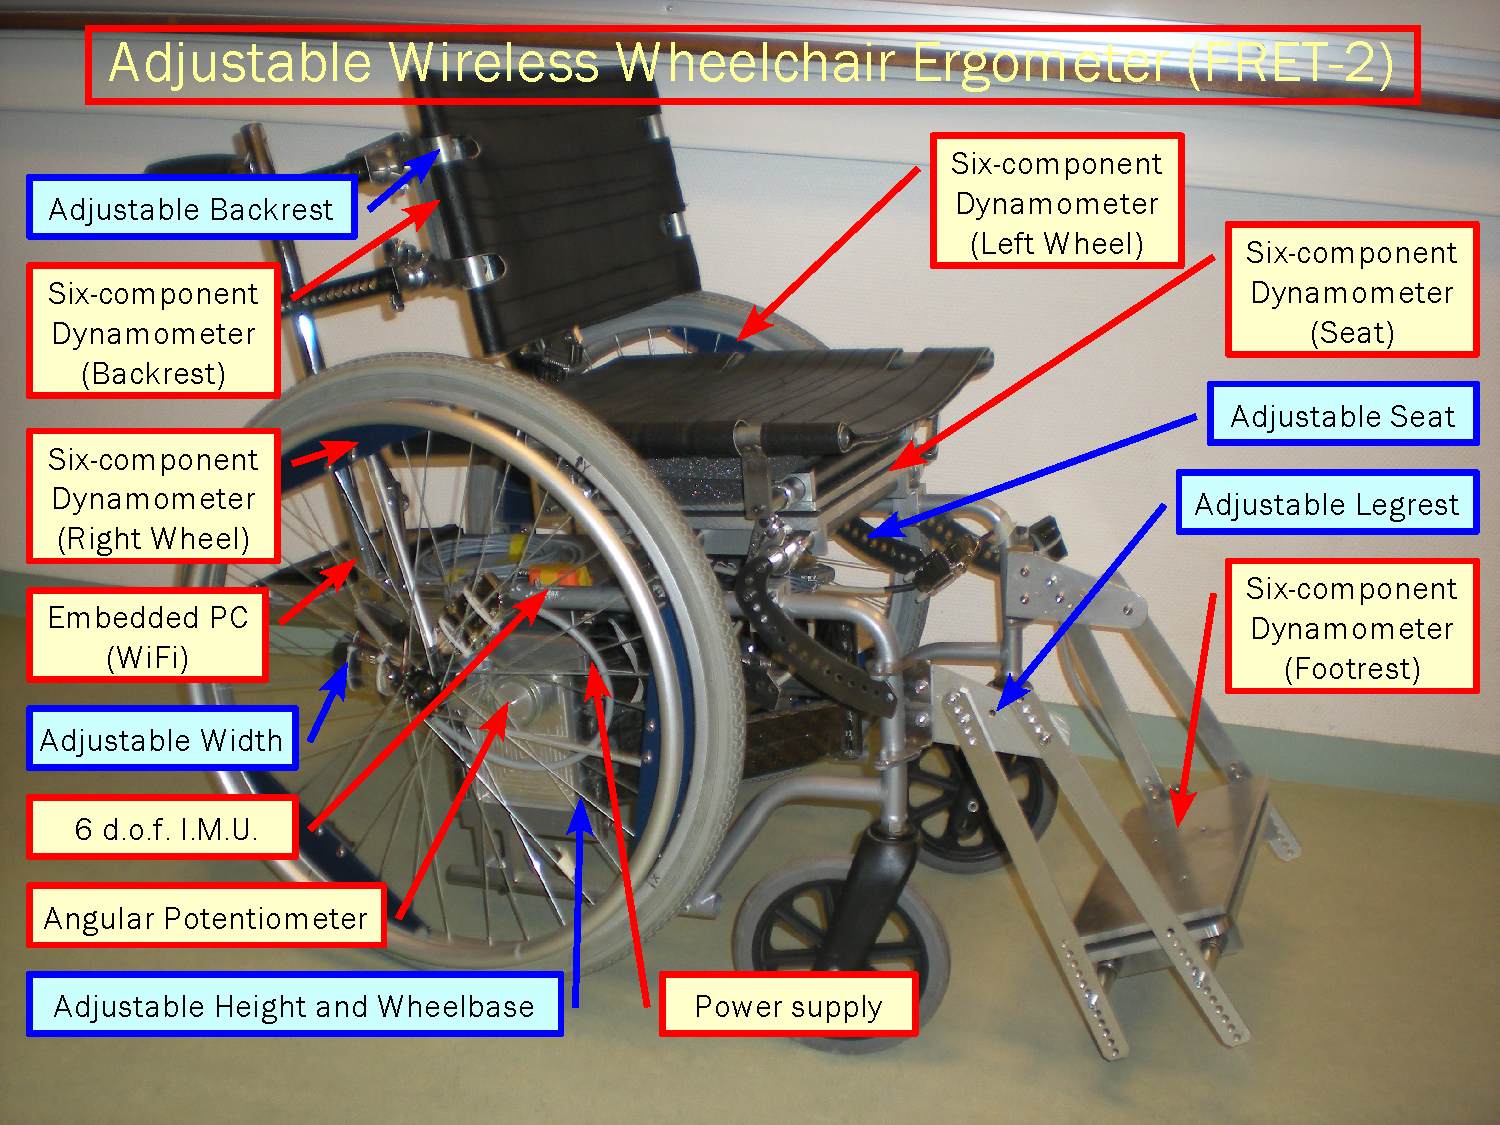
\includegraphics[scale = 0.4]{images/FRET-2_Legend_GB}
\caption{Captioned picture of the adjustable wireless wheelchair ergometer (FRET-2).}
\label{fret_legend}
\end{figure}


The measurements recorded by the sensors, which are the prupose of our analysis, consist of 44 attributes; of which 30 represent the dynamic parameters (Fx, Fy, Fz, Mx, My, Mz = 6 components x 5 dynamometers). The 14 other attributes represent the kinematic parameters of the MWC and its position relative to the Earth's magnetic North.

\section[Wheelchair time series]{Knowledge discovery on wheelchair time series}
After the construction ofthese measuring instruments (FRET-1 and FRET-2), they habe been used to measure the efforts made by MWC in actual conditions of wheelchair locomotion. Thus, several experiments have been conducted with several subjects,  where the efforts produced during actual wheelchair locomotion were measured with the FRET-2. The abundance of the recorded measurements highlighted the problem of the exploitation of these measures for knowledge extraction. Two main and complementary approaches can be used to analyze measurements from MWC locomotion. The first is to use mechanical models to calculate the physical parameters of motion and the second is to use data mining models to exploit measurements.  In this section, we present the contributions of these two approaches, which will allow us to position our work.



\paragraph{}Manual wheelchair locomotion causes significant mechanical stresses in the upper limbs. To remedy this problem, biomechanical studies have been conducted to identify and quantify traumatic factors such as:
\begin{itemize}
\item The doctoral thesis of Nicolas DE SAINT REMY (2005) \cite{Remy2005} who proposed a
mechanical model relating the forces applied to a MWC and its displacement ( Figure \ref{Wheelchair_model} ). This work particularly highlighted the fact that wheelchair acceleration is a function of subject's movements.

\begin{figure}[h]
\center
\includegraphics[scale = 0.6]{images/wheelchair_model2}
\caption{Balance of forces applied to a manual wheelchair during propulsion. For the clarity of the figure, the analysis of the movement of the {subject + MWC} system is reduced to that of the system's centre of gravity, G \cite{Remy2005}}
\label{Wheelchair_model}
\end{figure}

\item The doctoral thesis of Christophe SAURET (2010) \cite{Sauret2010} who proposed a method of calculating the mechanical power developed by manual wheelchair users to move. This model analyzes the kinetics of the {subject + MWC} system. For that purpose, the author developped a detailed kinematic model of the {subject + MWC} system (Figure \ref{Wheelchair_model2}) allowing to record their movements with a 3D motion analysis system during actual locomotion on the ground. 


\begin{figure}[h]
\center
\includegraphics[scale = 0.5]{images/squelette}
\caption{Markers for kinematic analysis of manual wheelchair locomotion\cite{Sauret2010}}
\label{Wheelchair_model2}
\end{figure}

\end{itemize}


\paragraph{} More and more works in the literature suggest using the tools developed in data mining for a better understanding of human locomotion. For example, in \cite{van2017future}, the authors ask whether advances in data science and technology could provide a different and perhaps more objective view of the analysis of wheelchair users' motor abilities. On one hand, technical advances have made it possible to measure the efforts made by wheelchair users during their movement using sensors. On the other hand, datamining models have been proposed and allow to perform several task on the data (clustering, classification, …). 

In \cite{faria2012patient} the authors explained how they used robotics and data mining knowledge to build an Intelligent Manual Wheelchair. which can be controlled from multiple interfaces: joysticks, facial expressions, voice commands, head movements.  Since Intelligent Wheelchair users have various characteristics, a series of tests have been carried out to classify them and to define profiles that allow the MWC to be adjusted appropriately for each user.

In \cite{athanasiou2009bayesian} the authors presented a model based on Bayesian networks to improve the medical treatment of patients in wheelchairs with a spinal cord injury. Indeed, the treatment of these patients  is based on the level of spinal cord injury and symptoms. A lesion in the spine has three consequences: an inconsistency of the bowel, an inconsistency of the bladder, a loss of the skin sensitivity. The higher the lesion, the more widespread its effects on patients are. Thus a patient with a low lesion will affect the patient's legs  and a patient with a high lesion will see his four limbs affected. Because of this loss of sensitivity, symptoms observed in the patient are often incomplete, which introduces uncertainty into the diagnosis that is captured by Bayesian networks and conditional probabilities.





\section{Conclusion}



Throughout this chapter, we showed that there is a large number of MWC users in the world and that it is crucial to analyze this particular means of locomotion to improve the living conditions of people moving in a MWC. We have presented the main tools designed and manufactured for wheelchair locomotion analysis and some previous works that used data mining mechanics models to improve the study of wheelchair locomotion or  to help help physicians to diagnose the adverse for the adverse effects treatment of spinal cord injury causing paralysis and requiring the use of MWC. 


In the scientific literature,  mechanical or data mining models are used for manual wheelchair locomotion analysis.  In this thesis, however, we want to \textbf{design} data mining models that is able to take into account both the specificities of MWC locomotion data and their use to analyze wheelchair locomotion from a new point of view. In the next chapter, are presented the existing works in the literature of knowledge extraction on time-series, which will allow us to identify and then choose  useful approaches for the analysis of wheelchair locomotion.






\begin{table}[ht]
\centering
\begin{tabular}{|l|}

\hline
\rowcolor{LavenderBlush}
Key points\\
$\bullet$ The first section of the chapter \ref{locomotion_analysis} presents the three central research questions related \\ to the analysis of Manual Wheelchair locomotion \\ \; We explain why this thesis is focused on the study and improvement of motor skills of\\ Manual Wheelchair users. \\
\\
$\bullet$ The second section of the chapter \ref{locomotion_analysis} presents the measurement tools built to measure \\ the efforts  made by manual wheelchair users during their locomotion. Here we insist on \\ the Wheelchair Field  ergometer, which  produces the time series that we use throughout \\ our work for  the analysis of manual wheelchair locomotion. \\
\\
$\bullet$ The third section of the chapter \ref{locomotion_analysis} presents the mechanical models and data mining models \\ used in the literature for manual wheelchair locomotion analysis.\\

\hline
\end{tabular}
\end{table}





\chapter{Knowledge discovery on time series}
\label{kdd}

\section{Introduction}

Datasets can be grouped into four main categories regarding their temporality \cite{roddick2002survey}: 
\begin{itemize}
\item Static datasets: these are datasets with no temporal context. We have for example the radius of a wheel, the circumference of a circle, the gravity in a place.
\item Sequences datasets: they consist of   ordered sequences of events. This category includes an order but not time. As an example, we can cite a DNA sequence (GTTTTCCCAGTCACGAC).
\item Time-indexed datasets: they consist of a set of temporal data sequences ; for example a set of measures taken at a more or less regular time interval.
\item Full-time data: Each tuple has one or more time components; time series belongs to this latter category.
\end{itemize}

Time series have several characteristic properties: usually, they are noisy, uncertain and  
they often have high dimensionality and high auto-correlation. Each of those features can interfere with the mining of time series.  To remedy this, preprocessing technics have been proposed in the literature.
\section{Preprocessing of time series}


\subsection{Denoising time series}
Several filters have been proposed in the literature to remove noise contained in time series. In this section, the most  frequently used filters are presented.
\paragraph{Kernel smoothing:} this filter refers to a statistical technique for recovery of underlying structure in data sets. Its basic principle is to estimate a real-valued function as the weighted average of neighboring observed data. The weight is defined by a function named kernel, such that closer points to real values are given higher weights \cite{wand1994kernel}.

\paragraph{Polynomial Regression:} this filter consists in fitting a nonlinear relationship between the values of an independent variable x (predictor variable)  and the corresponding conditional mean of y (variable to explain), denoted E(y |x). This filter has been used to describe nonlinear phenomena. More formally, polynomial regression is defined as the problem of finding a polynomial:  $g(x)=\beta_{0}+\beta_{1}x+...+\beta_{m}x^{m}$ of a certain degree $m$ for wich $E(Y-g(x))^{2}$ is as small as possible \cite{kendall1961advanced}.

\paragraph{Wiener-Kolmogorov Filtering of Short Stationary Sequences:}  
The idea of this filter is to produce a statistical estimate of the actual signal from the noisy signal. Using the Wiener-Kolmogorov filter assumes the knowledge of stationary signal, noise spectra, and additive noise \cite{pollock2007wiener}.

\paragraph{Filtering in the Frequency Domain:}   The purpose of frequency-based filters is to remove the noise contained in a signal. To achieve this goal, the signal is initially broken down into a set of frequencies using a Fourier transform. This set of frequencies is called the signal spectrum. Depending on the application, it may be appropriate to suppress high or low frequencies, or both, to suppress signal noise. These filters are generally named low-pass, high-pass, bandpass, or notch filter. These filters can also be combined in many ways: in cascade, in parallel, etc \cite{buttkus2012spectral}.

\paragraph{Kalman Filter and the Smoothing Algorithm,} also known as linear quadratic estimation (LQE), is a Bayesian estimation technique used to track stochastic dynamic systems being observed with noisy sensors. The filter produces estimates of unknown variables that tend to be more accurate than those based on a single measurement alone, by estimating a joint probability distribution over the variables for each timeframe. The algorithm works in two phases: extrapolation (prediction) and update (correction). In the extrapolation step, the Kalman filter produces estimates of the current state variables, along with their uncertainties, based on the previous state variables and their uncertainties. Once the outcome of the next measurement is observed, these estimates are updated using a weighted average, with a higher weight being given to estimates with higher certainty. The algorithm is recursive. It can run in real time, using only the current input measurements and the previously calculated state and its uncertainty matrix \cite{matthies1989kalman}.



\subsection{Reducing uncertainty}
Another important step of preprocessing time series is to reduce the uncertainty that they contained. For this purpose some transformations have been introduced in literature.


\paragraph{Uncertain moving average:}   For uncertain time series, each value is associated with a standard deviation representing uncertainty. The uncertain moving average (UMA) filter is then defined as the weighted average of the consecutive data points of a time series over a given time interval. The weights at each timestamp $i$ are calculated from the inverse of the uncertainty. Thus, in the calculation of the mean, a weight $(w)$ inversely proportional to the uncertainty will be given to each data point in the time series. Uncertain moving average returns times series: $x^{UMA}=<x_{1}^{UMA},...,x_{m}^{UMA}>$ for which $x_{i}^{UMA}=\frac{1}{2w+1}\stackrel[k=i-w]{i+w}{\sum}\frac{x_{k}}{\sigma_{k}},\,1\leq i\leq m$ \cite{Orang2015}.

\paragraph{Z-normalization} is used with uncertain moving average to reduce the advert effect of uncertainty in time series. In general, z-normalization improves similarity search quality, because it makes similarity measures invariant to scaling and shifting. Given an uncertain time series: $X=<X_{1},...,X_{m}>,$ its normal form: $\hat{X}=<\hat{X}_{1},...,\hat{X}_{m}>$ is defined as follows: 

\[
\ensuremath{\hat{X}_{i}}=\frac{X_{i}-\overline{X}}{S_{X}},
\]
where $\overline{X}$ and $S_{X}$ denote the sample mean and standard deviation of expected values of X, respectively \cite{Orang2015}. That is,

\[
\overline{X}=\frac{1}{n}\stackrel[i=1]{n}{\sum}E(X_{i}),
\]

\[
S_{X}=\sqrt{\frac{1}{(n-1)}\stackrel[i=1]{n}{\sum}(E(X_{i})-\overline{X})^{2}}.
\]

\subsection{Dimensionality reduction}
Time complexity of a mining time series algorithm depends on the length of the time series. Reducing dimensionality of time series allows reducing their processing time. To achieve this goal, many representations have been proposed and can be grouped into three main categories: 

\paragraph{Non-data-adaptive:}Dimension reduction methods are called non-data-adaptive because they take parameters of which value does not vary according to the considered data set. One of the first work in this family was done by Agrawal \\ \cite{Agrawal1993} who used a Discrete Fourier Transform to compress time series. In the same family, we can also cite the following time series representations:  Discrete Wavelet Transform (DWT) \cite{chan1999efficient}, Piecewise Linear Approximation (PLA) \cite{eriksson2004piecewise}, Piecewise Aggregate Approximation (PAA) \cite{Keogh2001a}. 

\paragraph{Data adaptive:} This family of time series representation  consists of methods that take the properties of the dataset into account when choosing the method parameters. All non-data-adaptive representations can be transformed into data-adaptive representations by adding a parameter selection method to them. As examples of data-adaptive representations, there is Adaptive Piecewise Constant Approximation (APCA) \cite{keogh2001locally} and Singular Value Decomposition (SVD) \cite{de1994singular} and Symbolic Aggregate Approximation (SAX) \cite{lin2003symbolic}.

\paragraph{Model based:} The assumption here is that time series are described by an underlying model.  Dimensionality reduction is achieved by identifying the model parameters that generate the time series. Several approaches use temporal parametric models such as statistical modeling by feature extraction \cite{Esling2012}, Auto Regressive Moving Average (ARMA) models \cite{kalpakis2001distance}, Markov Chains (MCs) and Hidden Markov Models (HMM) \cite{panuccio2002hidden}.
\\

After cleaning the time series, we are now ready to extrat relevant information from them. Several data mining tasks can be performed with time series.

\section{Similarity Measures}

Before performing data mining tasks, it is essentia to be able to compare time series. Most often,  similarity functions compare time series as humans would do. Indeed, without much of stretch, human recognition understand and look at the likenesses between two time series based on their amplitude, scale, temporal warping, noise, and outliers. As indicated by \cite{fu2011review} \\ \cite{ralanamahatana2005mining}  \cite{Esling2012}, any similarity measure  for time series comparison ought to be reliable with human recognition and perception and have the following properties:


\begin{itemize}
\item It should perceive perceptually comparative datasets even if  they are not mathematically identical;
\item It should resemble human intuition;
\item It should be able to capture global and local similarities;
\item It should have a universal meaning that is not restricted to particular type of time series datasets and do not assume some constraints on time series data;
\item It should be robust to distortions and set of transformations. More specifically it should be robust to amplitude
shifting, uniform amplification, uniform time scaling, dynamic amplification, dynamic time scaling, adding noise and outliers transformations or any combination of these transformations.
\end{itemize}
The latter property is also known as invariance.

\subsection{Time-Series Invariances}
In this section, we review common time-series distortions and their invariances. More detailed information can be found in \cite{batista2014cid}. 

\paragraph{Scaling and translation invariances:} We should be able to perceive the similarity of sequences in spite of contrasts in amplitude (scaling) and offset (translation). For instance, these invariances may be helpful to analyze seasonal variations in currency values on foreign trade markets without being biased by inflation.


\paragraph{Shift invariance:}  We should be able to recognize two similar sequences even if they vary in phase (global alignment) or when there are regions of the sequences that are aligned and others are not (local alignment). For instance, heartbeats can be out of phase depending on when we start recording, and handwritings of the same sentence from various people will require alignment depending on the size of the letters and on the spaces between words (local alignment).


\paragraph{Uniform scaling invariance:} We should be able to compare two sequences even if they have different length. To do so, sequences that differ in length require either extending of the shorter sequence or, contracting of the longer sequence. For instance, this invariance is required for  heartbeats recorded at different sample frequencies  (e.g.: 10, 50 ou 100 Hz).  

\paragraph{Occlusion invariance:} We should be able to compare two time series even if some of their sub-sequences  are missing; we can also compare the sequences by ignoring the sub-sequences that do not match well.  For example, suppose an archaeologist who has just found a skull in a research site, and  would like to determine to which species this skull belongs. Let us also suppose that we have a database of time series corresponding to the skulls of living species. We could then compare the time series from the found skull to those stored in the database. This comparison should be possible even if the found skull is damaged. In other words, we should be able to make a comparison even if the time series extracted from the found skull has missing sub-sequences.

\paragraph{Complexity invariance:} We should be able to recognize time series with similar shape even if they have different complexity.  For example, the same audio signals that were recorded indoors and outdoors might be considered similar, although outdoor signals will surely be noisier than indoor ones. 


\\

Depending on the application domain, some or all the invariances can be required for the comparison of time series. The preprocessing step can handle some of those invariances; for instance, z-normalization of time series allows their comparison to be scaling invariant. However, all invariances cannot be handled by preprocessing step and should then considered by more sophisticated distances or dissimilarities functions. In the next section, we review the most common of such distance measures.





\subsection{Categories of time series similarity function}


Time series similarity measures can be generally divided into following four main categories:

\\

\textbf{Based similarity function} compares two time-series based on the sum of the distances in a Euclidian space between data points of both times series located at approximately the same timestamp. By doing so, the distance between two time series with similar shapes will be low. On the opposite, the distance between time-series that have a different shapes will be high. In this family, there are Lp norm \cite{yi2000fast} \cite{keogh2003need}, and Dynamic time warping distance \cite{ MyersRabinerRosenberg1980} for instance. However, those distances are sensitive to noise.

\\

\textbf{Edit Based distance} allows evaluating the dissimilarity between two character strings. These dissimilarity functions are able to handle noisy regions and outliers. The principle of these similarity functions is the following: Edit based distances count the minimum number of operation necessary to transform a character string to another. Different edit based dissimilarity functions use different operations to transform one string to another. A well known edit based distance is Levenshtein distance. That uses three operations: suppression, insertion and substitution of letters. Edit based distances in time series domain are based on the same principle. Time series data points can be skipped during the comparison (deletion) or one  data point can be compared to several data points of the other time series (insertion). Among the well-known  edit based distances in time series domain we can cited: Longest Common SubSequence (LCSS) \cite{das1997finding}, Edit Distance on Real sequence (EDR) \cite{chen2005robust} and Time Warp Edit Distance (TWED) \cite{marteau2009time} algorithms. LCSS distance uses a threshold parameter for point matching as well as a warping threshold for allowing gaps for matching two time series. EDR is a variant of the edit distance for real-valued series. Opposite to LCSS, EDR assigns penalties based on the length of existing gaps between two series. TWED is a dynamic programming algorithm that introduces a parameter to control the elasticity measure along the time axis. 

\paragraph{Feature Based distance:} this distance has been designed to ensure some invariances such as rotation invariance. Time series can be compared based on their properties rather than on their shape. So, Feature Based similarity measures compare two time series by computing a feature set for
each time series that reflects their properties\footnote{We will use this type of distance later when analyzing manual wheelchair locomotion (Chap. \ref{application}).}. For example, DFT and DWT coefficients can be used to compare the similarity between time series \cite{shatkay1996approximate}.


\paragraph{Structure Based similarity measures:}These measures are designed to compare time series on a global scale based on their structure. The general principle of those similarity functions is to compare time series based on a high-level representation that captures global properties of the time series, such as histogram, for instance  \cite{lin2009finding}.   



\section{Datamining task on time series}
\paragraph{Indexing time series: }
The problem of indexing or query by content can be defined as follows: given a query time series Q, and some similarity/dissimilarity measure D(Q,C), find the most similar time series in database DB. When querying time series by content, a challenge consists in finding as fast as possible a time series in the database that is similar to the query. To achieve this goal, some dimensionality reduction technics have been used:  for instance, in \cite{Agrawal1993}, time series have been transformed into a more compact representation using  DFT before their comparison. Many other dimensionality reduction techniques have been used for the same purpose, such as Discrete Wavelet Transform (DWT) and Discrete Cosine Transform (DCT) \cite{chan1999efficient}. Other representation approaches used for query by content are PLA, PAA, APCA \cite{keogh2001locally}, and SAX \cite{Lin2007}. These latter authors \cite{Lin2007}  have shown that SAX outperforms other representations for query by content applications.

\paragraph{Motif Discovery:}
Time series motifs are pairs of individual time series, or subsequences of a longer time series, which are very similar to each other and carry precise information about the underlying source of the time series. The idea for motif discovery in time series is inspired from DNA analysis. When they exist, motifs can be used to construct meaningful clusters when clustering time series, which is the case of unsupervised shapelet algorithm \cite{ulanova2015scalable}. Associating each class with a motif can speed-up the classification of time series; this idea is used by the shapelet transform algorithm\footnote{We will use this type of distance later when analyzing manual wheelchair locomotion (Chap. \ref{training_technic} ).} \cite{lines2012shapelet}.

\paragraph{Anomaly Detection:}
Anomaly detection refers to the problem of finding patterns in data that do not conform to the expected behavior. These nonconforming patterns are often referred to as anomalies, outliers, discordant observations, exceptions, aberrations, surprises, peculiarities, or contaminants in different application fields. Among these, anomalies and outliers are two terms  most commonly used in the context of anomaly detection; sometimes interchangeably. Anomaly detection finds extensive use in a wide variety of applications such as fraud detection for credit cards, insurance, or healthcare, intrusion detection for cyber-security, fault detection in safety-critical systems, and military surveillance of enemy activities \cite{chandola2009anomaly}.

\paragraph{Temporal Association Rule Discovery:}
In a transactional database, association rules allow searching for items that often appear together in the same transaction. For instance, in the database of a Shop, the discovered rules will indicate, which products are often bought together. The association rules do not give any information on the precedence of the occurrence of one event concerning the other. Hence the need to define temporal association rules,  which are particularly appropriate as candidates for causal rules' analysis in temporally adorned medical data, such as in the histories of patients' medical visits. Patients are associated with both static properties, such as gender, and temporal properties, such as age or current medical treatments, any or all of which may be taken into account during mining \cite{Vasimalla2017}.

\paragraph{Summarization (Visualization):}
The problem of time series visualization or summarization can be defined as follows: given a time series $Q$ containing $n$ data points where, $n$ is an extremely large number, create a (possibly graphics) approximation of $Q$ which retains its essential features but fits on a single page, computer screen, executive summary. Summarization can be viewed as a higher level clustering of time series  where clusters are associated with text or graphical descriptions. Some famous approaches of time series summarization  are:
\begin{itemize}

\item    \textbf{Time searcher}: it is a query by content summarization tool. Here, a user specifies a set of constraints (intervals) graphically to which time series data points should belong. Those constraints are called time series boxes \\ \cite{hochheiser2003interactive}.
\item    \textbf{Calendar based visualization} of univariate time series data: its goal is to simultaneously identify patterns and trends on multiple time scales (days, weeks, seasons). To do so, Calendar based visualization first clustered similar daily data patterns and visualized the average patterns as graphs and the corresponding days on a calendar \cite{van1999cluster}. 
\item    The \textbf{spiral visualization} is appropriated with large data sets and supports much better than line graphs the identification of periodic structures in the data. Spiral visualization supports both the visualization of nominal and quantitative data based. The extension of the spiral visualization to 3D gives access to concepts for zooming and focusing and linking in the data set \cite{weber2001visualizing}. 
\item    \textbf{GrammarViz} is a visualization tool that allows efficient discovery of frequent and rare patterns  of variable length in time series. It is based on the symbolic representation of time series sax and context-free grammar \cite{senin2014grammarviz}.
\end{itemize} 

\paragraph{Prediction} or time series forecasting is one of the most useful data mining tasks on time series: for example, time series forecasting is used to predict the weather, the cost of an action in the stock exchange market, or early identified epidemiological risks and raised up alarms. A time series forecasting method is based on a mathematical model that capture the main characteristics of the time series like seasonality, periodicity, trend, and that can be used to guess unknown (or future) values of the time series. Many other algorithms used for time series forecasting are based on Auto-Regressive (AR) models. More sophisticated approaches are also used such as neural networks and cluster function approximation \cite{mahalakshmi2016survey}.
\paragraph{Classification:}
Classified time series consists of assigning an unlabelled time series to one, two or more classes. Many classification algorithms for time series have been proposed in the literature and can be gathered into four main groups
\begin{itemize}
\item \textbf{Dictionary classifiers}: generally, these classifiers first transform time series into characters strings that can be decomposed into a set of word or bag of words, a word being simply a subsequence of the characters string. Each time series is then described by the occurrence frequency of each word in it. The set of time series represented in the space of words is called a dictionary; The classification of time series is then based on the presence or absence of words in this dictionnary. Several algorithms of the literature are based on this principle, such as Bag of Patterns \cite{lin2012rotation},  SAX and Vector Space Model \cite{senin2013sax}, Bag of SFA Symbols(BOSS) \cite{schafer2015boss} and DTW Features\cite{kate2016using}.

\item \textbf{Classifier-based on the alignment of whole time series}: those classifiers are based on distance functions that operate over the entire length of the time series. The difference between the classifiers of this family is based in part on the characteristics of the distance functions used. These distance functions can be based on the shape of the time series (Derivative Dynamic Time Warping  \cite{keogh2001derivative}, Weighted Dynamic Time Warping  \cite{jeong2011weighted}, Complexity-Invariant Distance  \cite{batista2011complexity}), on their properties, on their structures or on their symbolic representation (Time Warp Edit Distance \cite{marteau2008time}, Move Split Merge \cite{stefan2013move}).

\item \textbf{Shapelets Classifiers:}  Unlike classifiers based on the comparison of the time series over their entire length, shapelets classifiers look for characteristic sub-sequences in time series called shapelet whose presence or absence indicates whether or not a time series belongs to a class. We have for example: Shapelet Transform \cite{lines2012shapelet}, Learned Shapelets \cite{grabocka2014learning}, Fast Shapelet Tree \cite{rakthanmanon2013fast}

\item \textbf{Intervals Classifiers:} The idea here is to find localized discriminatory features on time series based on some statistical properties calculated over intervals of variable length. A time series of length $m$ will have $ m(m-1)/2$ possible contiguous intervals. An interval associated with some statistical properties and a condition is a literal, which gives some information about what happened in an interval: for instance, is the mean of a sequence of data points greater or less than a define threshold? The classifier tries to find a relationship between what happened in an interval and  time series classes. Many classifiers are based on this principle, such as: Time Series Bag of Features  \cite{baydogan2013bag}, Time Series Forest  \cite{deng2013time}, Learned Pattern Similarity  \cite{baydogan2016time}.
\end{itemize}


\paragraph{Clustering:}
The clustering of time series consists of grouping them to build very homogeneous and well-separated groups under some similarity/dissimilarity measure D(Q, C) \cite{rani2012recent}. "Homogeneous" means that the intra-group variance is small and "Well separated" means that the inter-groups variance is high. There are many ways to categorize time series clustering algorithms depending on the \textbf{distance function} used, the \textbf{data transformation} or  the \textbf{clustering strategy}. 


When considering \textbf{distance function}, we have two categories of time series clustering algorithms: those that operate on the whole time series and those that operates on a sub-sequences of time series.


 When considering \textbf{data transformation}, we can  gather time series clustering algorithms into three groups:  raw data, feature-based and model-based clustering. 


When considering \textbf{clustering strategy}, we have five categories of clustering algorithms: 

\begin{itemize}
\item   \textbf{Distance-based} clustering, which is divided in two sub-categories:
	\begin{itemize}
	\item \textbf{Partitioning clustering algorithms}  partition the data in        	high dimensional space into multiple clusters. We have for example kMeans like 		algorithms (kMeans, kMedians, kMedoids, XMeans, KMeans++)
	\item \textbf{Hierarchical clustering algorithms} are grouped into two 				subcategories: \textbf{Agglomerative clustering algorithms} first consider each 		object of the dataset as a cluster and then try to merge clusters until  obtainning 		one cluster: it is a bottom-up merging strategy. \textbf{Divisive clustering 			algorithms} first considers that all the data points are in the same cluster 		and then try to split this cluster to obtain more homogenous ones: it is the top-down merging strategy.
	\end{itemize}
   
\item \textbf{Density-Based clustering and grid-based clustering algorithm}:
 
\begin{itemize}
	\item The principle of \textbf{density-based clustering} is the following:   given a time 		series that will be considered as the center of the cluster,  all the time series of the database that have a distance less or 		equal to a defined threshold to the center of the cluster are gathered. Thus, the 			algorithm splits the space into more or less dense regions; then small dense  			regions can be merged into more significant regions. This algorithm allows to identify  		clusters of arbitrary shapes  \cite{kriegel2011density}.
	\item \textbf{Grid-based clustering} divides the data space into a grid-like 				structure, which allows determining the characteristics of the data \cite{amini2011study}.
\end{itemize}


\item \textbf{Probabilistic and generative models} can be modelled  with a generative process assuming the data follow a particular distribution like a mixture of Gaussian. Then the model parameters are estimated using the expectation-maximization algorithm (EM), that consider the parameters that maximize the likelihood of the model to the data. On this basis we may estimate the generative probabilities that will be used to construct the generative model \cite{merugu2003privacy}.


\item  \textbf{High-dimensional clustering algorithms}: time series may be set in a high dimensional feature space. To cluster them, many methods have been proposed:

\begin{itemize}
	\item  \textbf{Subspace clustering}: Subspace clustering looks for a cluster in 	different subspaces of a dataset.  A subspace is a subset of the $d$ dimensions 		of a given dataset; all the dimensions of high dimensional data are not useful. 	Subspace clustering algorithm identifies relevant dimensions allowing them to 		find clusters. There are two main subspace clustering branches based on their 		search strategy. Top-down algorithms find an initial clustering in the full set 		of dimensions and evaluate the subspaces of each cluster, iteratively improving 	the results. Bottom-up approaches find dense regions in low dimensional spaces 		and combine them to form clusters \cite{parsons2004subspace}.
	\item \textbf{Dimensionality reduction}: many dimensionality reduction 				techniques have been proposed for clustering purpose. A well-known one is co-clustering, which consists of simultaneously clustering  columns (or dimensions) 	and	rows (data points) of a matrix \cite{dhillon2003information}.
	\item \textbf{Probabilistic latent semantic indexing (PLSI)} and \textbf{laten 		dirichlet allocation (LDA)}  are typical clustering techniques for text data. Indeed, text can be clustered in multiple topics and  each topic can be associated with a 		set of words (or dimension) or a set of rows (documents) can be simultaneously associated 			\cite{hofmann2017probabilistic}.
	\item \textbf{Nonnegative matrix factorization} is a kind of co-clustering 			algorithm. It proceeds as follows: a nonnegative matrix X \in $\mathbb{R}^{M			\times N}$ can be 			factorised into two lower rank matrices U \in $			\mathbb{R}^{M\times L}$ and V \in $\mathbb{R}^{L\times N}$ with $L < M$ and $L 		< N$.  The idea here is to identify clusters using the matrix $U$ which has a lower 	dimension than $X$  						\cite{wang2013nonnegative}.
	\item \textbf{Spectral clustering}: the principle is to cluster time series or 		data objects based on the spectrum of their similarity matrix. The spectrum 			being used here for dimensionality reduction  \cite{filippone2008survey}.
	
\end{itemize}
 

\end{itemize}
In the context of this thesis, the analysis of manual wheelchair locomotion implies to grouping  manual wheelchair users with similar motor abilities, based on measurements made during their locomotion in actual conditions: this approach is  equivalent to time series clustering. Several clustering algorithms proposed in the literature are harmonious compositions, consisting of a representation of time series, an adequate distance function and an appropriate clustering strategy as illustrated in the Tables \ref{tab:1}, \ref{tab:2} and \ref{tab:3}. Detailed informations is presented in \cite{rani2012recent}. 

 
 
\begin{landscape}
% Please add the following required packages to your document preamble:
% \usepackage[normalem]{ulem}
% \useunder{\uline}{\ul}{}
\begin{table}[ht]
\centering
\small
\caption{Temporal-Proximity-Based Clustering Approach}
\label{tab:1}
\begin{tabular}{|l|l|l|l|}
\hline
\multicolumn{1}{|c|}{\textbf{Paper}}                           & \multicolumn{1}{c|}{\textbf{Distance Measure}}                                                                                               & \multicolumn{1}{c|}{\textbf{Algorithm}}                                                  & \multicolumn{1}{c|}{\textbf{Application}}                                                       \\ \hline
M. Kumar                                                       & \begin{tabular}[c]{@{}l@{}}Based      on      the      assumed  independent   \\   Gaussian models   of\\   data errors\end{tabular} & Agglomerative Hierarchical                                                               & Seasonality pattern in retails                                                                  \\ \hline
T.-W. Liao                                                     & \begin{tabular}[c]{@{}l@{}}Euclidean      and    symmetric\\   version    of    Kullback–Liebler\\   distance\end{tabular}             & \begin{tabular}[c]{@{}l@{}}K-Means\\   and Fuzzy C-Means\end{tabular}                    & Battle simulations                                                                              \\ \hline
T.-W. Liao                                                     & Dynamic Time Warping                                                                                                                         & \begin{tabular}[c]{@{}l@{}}K-Medoids    Based     Genetic\\   Clustering\end{tabular} & Battle simulations                                                                              \\ \hline
C.S. Möller-Levet                                              & \begin{tabular}[c]{@{}l@{}}Short     time     series     (STS)   distance\end{tabular}                                                     & Modified Fuzzy C-Means                                                                   & DNA microarray                                                                                  \\ \hline
Shumway                                                        & \begin{tabular}[c]{@{}l@{}}Kullback–Leibler\\   discrimination         information measure\end{tabular}                                      & Agglomerative Hierarchical                                                               & \begin{tabular}[c]{@{}l@{}}Earthquakes     and     mining  explosions\end{tabular}   \\ \hline
Vit Niennattrakul                                              & Dynamic Time Warping                                                                                                                         & K-Means, K-Medoids                                                                       & \begin{tabular}[c]{@{}l@{}}Multimedia time\\   series\end{tabular}                              \\ \hline
\begin{tabular}[c]{@{}l@{}}Pooya Sobhe\\   Bidari\end{tabular} & Pearson Correlation                                                                                                                          & K-Means, Fuzzy C-Means                                                                   & Pattern extraction in genes                                                                     \\ \hline
Hardy Kremer                                                   & Dynamic Time Warping                                                                                                                         & \begin{tabular}[c]{@{}l@{}}Density   Based \\    Subsequence\\   Clustering\end{tabular} & \begin{tabular}[c]{@{}l@{}}Detecting climate\\   change\end{tabular}                            \\ \hline
Jian Yin                                                       & Grey Relation                                                                                                                                & Hierarchical Clustering                                                                  & \begin{tabular}[c]{@{}l@{}}Change  trend  of\\    traffic  flow  data\end{tabular}       \\ \hline
S. Chandrakala                                                 & Euclidean                                                                                                                                    & Kernal DBScan                                                                            & \begin{tabular}[c]{@{}l@{}}Multivariate       time     \\    series\\   clustering\end{tabular} \\ \hline
Aurangzeb Khan                                                 & Euclidean                                                                                                                                    & \begin{tabular}[c]{@{}l@{}}K-Mean+ MFP(Most Frequent\\   Pattern)\end{tabular}           & Stock and inventory data                                                                        \\ \hline
Mengfan Zhang                                                  & \begin{tabular}[c]{@{}l@{}}CVT(Computational          Verb\\   Theory)\end{tabular}                                                          & K-Means                                                                                  & Stock market data                                                                               \\ \hline
S.R.Nanda                                                      & Euclidean                                                                                                                                    & K-Means                                                                                  & Portfolio management                                                                            \\ \hline
Jianfei Wu                                                     & N/A                                                                                                                                          & K-Means                                                                                  & Stock data                                                                                      \\ \hline
\end{tabular}
\end{table}
\end{landscape}



\begin{landscape}
\begin{table}[ht]
\centering
\small
\caption{Representation-Based Clustering Approach Paper}
\label{tab:2}
\begin{tabular}{|l|l|l|l|l|}
\hline
\multicolumn{1}{|c|}{\textbf{Paper}} & \multicolumn{1}{c|}{\textbf{Features}}                                     & \multicolumn{1}{c|}{\textbf{\begin{tabular}[c]{@{}c@{}}Distance\\   Measure\end{tabular}}}                                    & \multicolumn{1}{c|}{\textbf{Clustering Algorithm}}                                 & \multicolumn{1}{c|}{\textbf{Application}}                                              \\ \hline
T.-C. Fu                             & \begin{tabular}[c]{@{}l@{}}Perceptually important\\   points\end{tabular}  & \begin{tabular}[c]{@{}l@{}}Sum of the mean\\   squared distance along the\\   vertical and horizontal\\   scales\end{tabular} & Modified SOM                                                                       & Hong Kong stock market                                                                 \\ \hline
M. Vlachos                           & \begin{tabular}[c]{@{}l@{}}Haar wavelet\\   transform\end{tabular}         & Euclidean                                                                                                                     & Modified k-means                                                                   & Non-specific                                                                           \\ \hline
Huiting Liu                          & \begin{tabular}[c]{@{}l@{}}Empirical mode\\   decomposition\end{tabular}   & Euclidean                                                                                                                     & \begin{tabular}[c]{@{}l@{}}Forward propagation\\   learning algorithm\end{tabular} & Non-specific                                                                           \\ \hline
Chonghui GUO                         & \begin{tabular}[c]{@{}l@{}}Independent component\\   analysis\end{tabular} & Euclidean                                                                                                                     & Modified k-means                                                                   & \begin{tabular}[c]{@{}l@{}}Real world stock time-\\   series\end{tabular}              \\ \hline
Jian Xin Wu                          & \begin{tabular}[c]{@{}l@{}}Independent component\\   analysis\end{tabular} & N/A                                                                                                                           & \begin{tabular}[c]{@{}l@{}}support vector\\   regression\end{tabular}              & Financial time-series                                                                  \\ \hline
Geert Verdoolaege                    & Wavelet transform                                                          & \begin{tabular}[c]{@{}l@{}}Kullback- Liebler\\   divergence\end{tabular}                                                      & k-means                                                                            & \begin{tabular}[c]{@{}l@{}}Detection of activated\\   voxels in FMRI data\end{tabular} \\ \hline
Liu Suyi                             & Hough transform                                                            & N/A                                                                                                                           & Mean shift algorithm                                                               & \begin{tabular}[c]{@{}l@{}}Feature recognition of\\   underwater images\end{tabular}   \\ \hline
Dong Jixue                           & Wavelet transform                                                          & N/A                                                                                                                           & \begin{tabular}[c]{@{}l@{}}Grid-based partitioning\\   method\end{tabular}         & Financial time-series                                                                  \\ \hline
\end{tabular}
\end{table}
\end{landscape}


\begin{landscape}
\begin{table}[ht]
\centering
\small
\caption{Model-Based Clustering Approach}
\label{tab:3}
\begin{tabular}{|l|l|l|l|l|}
\hline
\multicolumn{1}{|c|}{\textbf{Paper}} & \multicolumn{1}{c|}{\textbf{Model}}                                                     & \multicolumn{1}{c|}{\textbf{Distance measure}}                      & \multicolumn{1}{c|}{\textbf{\begin{tabular}[c]{@{}c@{}}Clustering\\   algorithm\end{tabular}}} & \multicolumn{1}{c|}{\textbf{Application}}                                              \\ \hline
Baragona                             & ARMA                                                                                    & \begin{tabular}[c]{@{}l@{}}Cross-correlation\\   based\end{tabular} & \begin{tabular}[c]{@{}l@{}}Tabu    search,  \\    GA\\   and\end{tabular}                      & Non-specific                                                                           \\ \hline
K. Kalpakis                          & AR                                                                                      & Euclidean                                                           & Partitioning   around medoids                                                                  & Public data                                                                            \\ \hline
Xiong and Yeung                      & ARMA mixture                                                                            & Log-liklihood                                                       & EM learning                                                                                    & Public data                                                                            \\ \hline
L. Wang                              & Discrete HMM                                                                            & Log-liklihood                                                       & EM learning                                                                                    & \begin{tabular}[c]{@{}l@{}}Tool        \\    condition\\   monitoring\end{tabular}     \\ \hline
Xin Huang                            & \begin{tabular}[c]{@{}l@{}}Fuzzy  set\\    and\\    R/S\\   analysis model\end{tabular} & N/A                                                                 & \begin{tabular}[c]{@{}l@{}}Fuzzy     \\    clustering iteration method\end{tabular}            & \begin{tabular}[c]{@{}l@{}}Predicting\\   agriculture drought\end{tabular}             \\ \hline
Shan Gao                             & ARMA-ARCH                                                                               & N/A                                                                 & N/A                                                                                            & \begin{tabular}[c]{@{}l@{}}To analyze the\\   effects of wind data series\end{tabular} \\ \hline
\end{tabular}
\end{table}
\end{landscape}


\section{Conclusion}
Time series are ubiquitous in science and are more and more used in the analysis of human locomotion. This chapter presents a general framework for extracting knowledge from time series, starting by time series pre-processing, which allows reducing the advert effects of noise, uncertainty, and dimensionality. Then, we present strategies that are used to compare time series, and we finally present data mining tasks on time series. This chapter presents what has been already done in the literature and raises the question of extracting relevant information from time series coming from wheelchair locomotion. The following chapters present some new strategies that we introduce and that are adapted to characteristics of time series issued from manual wheelchair locomotion.

\begin{table}[ht]
\centering
\begin{tabular}{|l|}

\hline
\rowcolor{LavenderBlush}
Key points\\
We highlight the different models of data mining present in the literature that could\\ be useful to our work, particularly for  \\
\\
$\bullet$ Pre-processing of time series (noise reduction, dimensionality reduction) \\
$\bullet$ Comparison of time series.\\ 
$\bullet$ The different data mining tasks performed on time series.\\
\hline
\end{tabular}
\end{table}